
    \begin{enumerate}

        \item \textbf{Colección}: Su llave primaria es el atributo \textit{nombre}, con dominio \textit{varchar} con una restricción de integridad de entidad (\textbf{NOT NULL}, \textbf{UNIQUE}). Sus atributos \textit{descripción}, \textit{tipo} y \textit{contacto} operan bajo el dominio \textit{varchar} con restricción \textbf{NOT NULL}.

        \item \textbf{Telefono\_Coleccion}: Se crea a partir de un atributo multivaluado de Colección, entonces su llave es compuesta por la llave de Colección y \textit{teléfono}. El atributo \textit{nombre\_coleccion} (dominio \textit{varchar}) actúa simultáneamente como llave foránea (\textbf{FK}) hacia la relación Colección, aplicando una restricción de integridad referencial. El atributo \textit{telefono} pertenece al dominio \textit{varchar} con restricción de dominio (\textbf{NOT NULL}).

        \item \textbf{Interactuar}: Al ser una relación muchos a muchos se crea esta tabla cuya llave primaria es compuesta por las llaves de las entidades participantes: \textit{nombre\_coleccion} e \textit{idMuseo}. El atributo \textit{nombre\_coleccion} (\textit{varchar}) funciona como llave foránea (\textbf{FK}) hacia la relación Colección, mientras que el atributo \textit{idMuseo} (\textit{int}) funciona como llave foránea (\textbf{FK}) hacia la relación Museo. Ambas imponen restricciones de integridad referencial.

        \item \textbf{Museo}: Su llave primaria es \textit{idMuseo}, perteneciente al dominio de los enteros (\textit{int}) y cuenta con una restricción de integridad de entidad (\textbf{NOT NULL}, \textbf{UNIQUE}). El atributo compuesto Dirección fue descompuesto en sus componentes indivisibles: \textit{calle}, \textit{numero}, \textit{cp} y \textit{estado}. Todos estos atributos, al igual que el atributo descriptivo \textit{nombre}, operan bajo el dominio de cadena de caracteres (\textit{varchar}), bajo restricciones de integridad de dominio (\textbf{NOT NULL}).

        \item \textbf{Teléfono\_Museo}: Se crea a partir del atributo multivaluado \textit{teléfono} de Museo. Su llave es compuesta por la llave \textit{idMuseo} (con dominio \textit{int}) con restricción de integridad referencial; y su llave principal \textit{teléfono} (con dominio \textit{varchar}) con restricción \textbf{NOT NULL}.

        \item \textbf{Obra}: Esta tabla se debe conservar por eficiencia, pues tiene un atributo multivaluado y dos especializaciones. Su llave primaria es \textit{idObra}, perteneciente al dominio de los enteros (\textit{int}) con una restricción estricta de integridad de entidad (\textbf{NOT NULL}, \textbf{UNIQUE}). Sus atributos \textit{titulo}, \textit{descripcion} y \textit{tipo} pertenecen al dominio \textit{varchar}, contando con restricciones de integridad de dominio (\textbf{NOT NULL}). Al tener una cardinalidad de 1:N con participación total en sus asociaciones con Museo, Colección y Artista, la tabla absorbe las llaves de esas 3 entidades. Entonces, integra tres llaves foráneas (\textbf{FK}): \textit{idMuseo} (\textit{int}) derivada de la relación Poseer, \textit{nombre\_coleccion} (\textit{varchar}) derivada de Tener, y \textit{nombre\_artista}, \textit{paterno\_artista}, \textit{materno\_artista} (todos \textit{varchar}) derivados de Crear (las 3 con restricción de integridad referencial).

        \item \textbf{Material\_Obra}: Se creó a partir del atributo multivaluado (\textit{material}) en Obra, por eso tiene una llave compuesta por la llave de Obra y \textit{material}. El atributo \textit{idObra} pertenece al dominio de los enteros (\textit{int}) y actúa simultáneamente como llave foránea (\textbf{FK}) hacia la relación Obra, aplicando una restricción de integridad referencial. El atributo \textit{material} adopta el dominio de cadena de caracteres (\textit{varchar}) con una restricción de integridad de dominio (\textbf{NOT NULL}).

        \item \textbf{Exhibir}: Esta tabla surge de la conversión de una cardinalidad de muchos a muchos (M:N) entre las entidades Obra y Exhibición. Su llave primaria es compuesta por los identificadores de las entidades que conecta: \textit{idObra} e \textit{idExhibicion}. El atributo \textit{idObra} (\textit{int}) y el atributo \textit{idExhibicion} (\textit{int}) fungen simultáneamente como llaves foráneas (\textbf{FK}) hacia sus respectivas relaciones de origen, con restricciones de integridad referencial. Finalmente, se incorporan los atributos de la relación, \textit{fecha\_inicio} y \textit{fecha\_fin}, operando ambos bajo el dominio \textit{date} con restricción de integridad de dominio (\textbf{NOT NULL}).

        \item \textbf{Especialización parcial disjunta}: El modelo conceptual presenta una jerarquía de especialización para la entidad Obra basada en su clasificación física (Pintura, Escultura, Miscelanea). Esta jerarquía se identifica como parcial disjunta. Por eso se crea una tabla para cada una de las tres subentidades. Cada nueva tabla incorpora como llave primaria el atributo \textit{idObra} (\textit{int}). Este identificador actúa simultáneamente como llave foránea (\textbf{FK}) hacia la superentidad Obra, estableciendo una restricción de integridad referencial. La Escultura recibe los atributos \textit{estilo} y \textit{dimensiones} (\textit{varchar}), así como el atributo físico \textit{peso} (\textit{decimal}); Pintura recibe \textit{estilo} y \textit{genero} (\textit{varchar}); y Miscelanea recibe \textit{pais} y \textit{formato} (\textit{varchar}). Todos estos atributos operan con una restricción de integridad de dominio (\textbf{NOT NULL}).

        \item \textbf{Tecnica\_Pintura}: Esta tabla se crea a partir del atributo multivaluado (\textit{técnica}) de Pintura. Su llave primaria es compuesta y está integrada por \textit{idObra} y \textit{tecnica}. El atributo \textit{idObra} (\textit{int}) actúa al mismo tiempo como llave foránea (\textbf{FK}) hacia la relación Pintura, aplicando una restricción de integridad referencial. El atributo \textit{tecnica} adopta el dominio \textit{varchar} con restricción de integridad de dominio (\textbf{NOT NULL}).

        \item \textbf{Especialización total disjunta}: El modelo E-R presenta una segunda jerarquía de especialización para la entidad Obra, clasificada por su estatus de propiedad en las subentidades Permanente y Prestada. A diferencia de la clasificación física, esta jerarquía se identifica como una especialización total disjunta. Las tablas resultantes, Permanente y Prestada, incorporan como llave primaria a \textit{idObra} (\textit{int}), la cual funciona simultáneamente como llave foránea (\textbf{FK}) hacia la superentidad Obra. Esta llave asegura la integridad referencial. La tabla Permanente aloja los atributos \textit{costo} (\textit{decimal}) y \textit{fecha\_adq} (\textit{date}). Por su parte, la tabla Prestada aloja el atributo \textit{prestador} (\textit{varchar}) y los atributos temporales \textit{fecha\_pres} y \textit{fecha\_dev} (ambos de dominio \textit{date}). Todos los atributos atómicos en ambas tablas operan bajo una restricción de integridad de dominio estricta (\textbf{NOT NULL}).

        \item \textbf{Artista}: Su llave principal es \textit{NombreC}, el cual es un atributo compuesto por \textit{Nombre}, \textit{Paterno} y \textit{Materno}, entonces su llave son esos 3 atributos. Todos adoptan el dominio \textit{varchar} con restricción de integridad de entidad (\textbf{NOT NULL}). Los atributos temporales \textit{nacimiento} y \textit{defuncion} se asignan al dominio \textit{date}, mientras que los atributos descriptivos \textit{pais}, \textit{epoca} y \textit{descripcion} operan bajo el dominio de cadena de caracteres (\textit{varchar}). Todos los atributos aplican una restricción de integridad de dominio para evitar valores nulos.

        \item \textbf{Estilo\_Artista}: Se crea a partir del atributo multivaluado \textit{estilo} de Artista. Su llave primaria es compuesta, uniendo el identificador completo de la entidad fuerte dominante (\textit{nombre}, \textit{paterno}, \textit{materno}) con su propio discriminante (\textit{estilo}). Los tres atributos que conforman el nombre fungen simultáneamente como llave foránea (\textbf{FK}) hacia la relación Artista, aplicando integridad referencial. El atributo \textit{estilo} adopta el dominio \textit{varchar} con restricción de integridad de dominio (\textbf{NOT NULL}).

        \item \textbf{Exhibición}: Su llave primaria es \textit{idExhibicion}, la cual se define bajo el dominio de los enteros (\textit{int}) con una restricción estricta de integridad de entidad (\textbf{NOT NULL}, \textbf{UNIQUE}). Su atributo \textit{titulo} pertenece al dominio de cadena de caracteres (\textit{varchar}) y opera con una restricción de integridad de dominio (\textbf{NOT NULL}).

    \end{enumerate}

    \begin{figure}[htbp]
        \centering
        % Ajusta el 0.9 al tamaño que prefieras (ej. 1.0 para ocupar todo el ancho)
        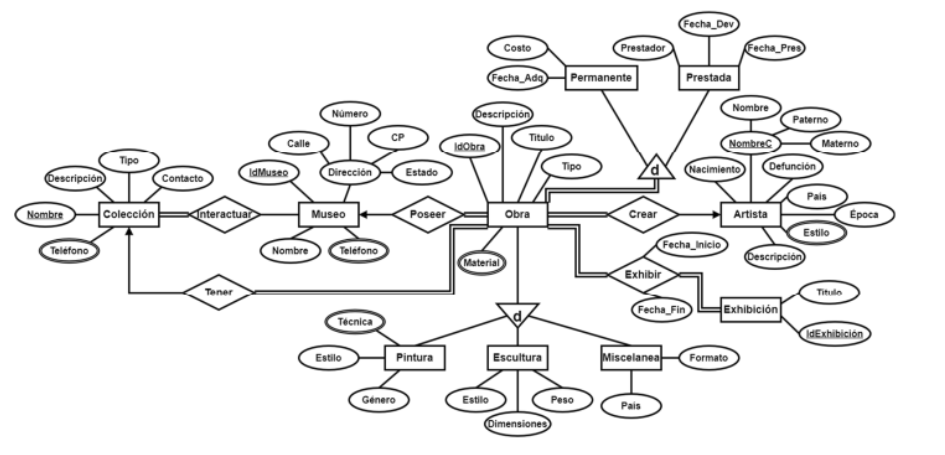
\includegraphics[width=0.9\textwidth]{Figuras/ER_2a.png}
        \caption{Modelo E-R correspondiente al inciso a).}
        \label{Modelo E-R inciso a}
    
    \end{figure}

    \begin{figure}[htbp]
        \centering
        % Ajusta el 0.9 al tamaño que prefieras (ej. 1.0 para ocupar todo el ancho)
        \includegraphics[width=0.9\textwidth]{Diagramas/2_a.drawio.png}
        \caption{Modelo Relacional correspondiente al inciso a).}
        \label{fig:modelo_relacional}
    
    \end{figure}

    \newpage

